% Options for packages loaded elsewhere
\PassOptionsToPackage{unicode}{hyperref}
\PassOptionsToPackage{hyphens}{url}
\PassOptionsToPackage{dvipsnames,svgnames*,x11names*}{xcolor}
%
\documentclass[
  11pt,
]{article}
\usepackage{lmodern}
\usepackage{amssymb,amsmath}
\usepackage{ifxetex,ifluatex}
\ifnum 0\ifxetex 1\fi\ifluatex 1\fi=0 % if pdftex
  \usepackage[T1]{fontenc}
  \usepackage[utf8]{inputenc}
  \usepackage{textcomp} % provide euro and other symbols
\else % if luatex or xetex
  \usepackage{unicode-math}
  \defaultfontfeatures{Scale=MatchLowercase}
  \defaultfontfeatures[\rmfamily]{Ligatures=TeX,Scale=1}
\fi
% Use upquote if available, for straight quotes in verbatim environments
\IfFileExists{upquote.sty}{\usepackage{upquote}}{}
\IfFileExists{microtype.sty}{% use microtype if available
  \usepackage[]{microtype}
  \UseMicrotypeSet[protrusion]{basicmath} % disable protrusion for tt fonts
}{}
\makeatletter
\@ifundefined{KOMAClassName}{% if non-KOMA class
  \IfFileExists{parskip.sty}{%
    \usepackage{parskip}
  }{% else
    \setlength{\parindent}{0pt}
    \setlength{\parskip}{6pt plus 2pt minus 1pt}}
}{% if KOMA class
  \KOMAoptions{parskip=half}}
\makeatother
\usepackage{xcolor}
\IfFileExists{xurl.sty}{\usepackage{xurl}}{} % add URL line breaks if available
\IfFileExists{bookmark.sty}{\usepackage{bookmark}}{
\usepackage{hyperref}
}
\hypersetup{
  pdftitle={Web et Interaction Homme Machine, programmation côté serveur},
  pdfauthor={Première NSI, Lycée du Parc},
  colorlinks=true,
  linkcolor=Maroon,
  filecolor=Maroon,
  citecolor=Blue,
  urlcolor=Blue,
  pdfcreator={LaTeX via pandoc}}
\urlstyle{same} % disable monospaced font for URLs
\usepackage[top=20mm,left=20mm,right=20mm,heightrounded]{geometry}
\usepackage{listings}
\newcommand{\passthrough}[1]{#1}
\lstset{defaultdialect=[5.3]Lua}
\lstset{defaultdialect=[x86masm]Assembler}
\usepackage{graphicx}
\makeatletter
\def\maxwidth{\ifdim\Gin@nat@width>\linewidth\linewidth\else\Gin@nat@width\fi}
\def\maxheight{\ifdim\Gin@nat@height>\textheight\textheight\else\Gin@nat@height\fi}
\makeatother
% Scale images if necessary, so that they will not overflow the page
% margins by default, and it is still possible to overwrite the defaults
% using explicit options in \includegraphics[width, height, ...]{}
\setkeys{Gin}{width=\maxwidth,height=\maxheight,keepaspectratio}
% Set default figure placement to htbp
\makeatletter
\def\fps@figure{htbp}
\makeatother
\setlength{\emergencystretch}{3em} % prevent overfull lines
\providecommand{\tightlist}{%
  \setlength{\itemsep}{0pt}\setlength{\parskip}{0pt}}
\setcounter{secnumdepth}{5}

\title{Web et Interaction Homme Machine, programmation côté serveur}
\author{Première NSI, \href{https://frederic-junier.org/}{Lycée du
Parc}}
\date{}

%%%jolis boites

\usepackage{fancybox, graphicx}



%%%%%%%%%%%%%%%%Packages et Macros Frederic%%%%%%%%%%%%%%%%%%%%%%%%%%%%%


%%%%Insertion de liens hypertextes %%%%

            
%%%%%%%%%%PSTricks%%%%%%%%%%%%

\usepackage{pstricks,pst-plot,pst-text,pst-tree,pst-eps,pst-fill,pst-node,pst-math,pstricks-add,pst-xkey,pst-eucl}


%%%%%%%Tikz%%%%%%%%%%%%%%%
\usepackage{pgf,tikz,tkz-tab}
% Pour les tableaux de signes ou de variations avec tkz-tab voir https://zestedesavoir.com/tutoriels/439/des-tableaux-de-variations-et-de-signes-avec-latex/#1-13389_tikz-un-package-qui-en-a-dans-le-ventre
\usetikzlibrary{arrows}
\usetikzlibrary{shapes.geometric}
\usetikzlibrary{shapes.geometric}
\usetikzlibrary{petri}
\usetikzlibrary{decorations}
\usetikzlibrary{arrows}
\usetikzlibrary{math}
 %Variables must be declared in a tikzmath environment but
       % can be used outside
%       \tikzmath{int \n; \n = 508; \x1 = 1; \y1 =1; 
%                   %computations are also possible
%                    \x2 = \x1 + 1; \y2 =\y1 +3; } 


%%%%%%%%%%%%%%%%%%%%%%%%%%%%%%%%%%%%%%%%
%%%%%%%%%%%Commandes Tikz Perso%%%%%%%%%%%%%%%

% Définition des nouvelles options xmin, xmax, ymin, ymax
% Valeurs par défaut : -3, 3, -3, 3
\tikzset{
xmin/.store in=\xmin, xmin/.default=-3, xmin=-3,
xmax/.store in=\xmax, xmax/.default=3, xmax=3,
ymin/.store in=\ymin, ymin/.default=-3, ymin=-3,
ymax/.store in=\ymax, ymax/.default=3, ymax=3,
}
% Commande qui trace la grille entre (xmin,ymin) et (xmax,ymax)
\newcommand {\grille}[2]
{\draw[help lines,black, thick] (\xmin,\ymin) grid[xstep=#1, ystep=#2] (\xmax,\ymax);}
% Commande \axes
\newcommand {\axes} {
\draw[->,very thick] (\xmin,0) -- (\xmax,0);
\draw[->,very thick] (0,\ymin) -- (0,\ymax);
\draw (0.95*\xmax, 0) node[above] {};
\draw (0, 0.95*\ymax) node[left] {};
}
% Commande qui limite l?affichage à (xmin,ymin) et (xmax,ymax)
\newcommand {\fenetre}
{\clip (\xmin,\ymin) rectangle (\xmax,\ymax);}

%Exemple d'utilisation

%\begin{center}
%\begin{tikzpicture} [xmin=-2,xmax=2,ymin=0,ymax=5]
%\grille{1} \axes \fenetre
%\draw plot[smooth] (\x,\x^2);
%\end{tikzpicture}
%\end{center}

%style pour la perspective cavalière française
%voir Tikz pour l'impatient page 68
\tikzset{math3d/.style=
{x= {(-0.353cm,-0.353cm)}, z={(0cm,1cm)},y={(1cm,0cm)}}}

%%%%%%%Symbole pour code calculatrice%%%%%%

%Flèche remplie pour défilement de menu

\newcommand{\flechefillright}{

\begin{tikzpicture}[scale=0.15] \fill (0,0)--(2,1)--(0,2)--cycle;
\end{tikzpicture}}

%%%%%%%%%%%%%Symboles pour calculatrice Casio%%%%
\newcommand{\execasio}{\Pisymbol{psy}{191}} %Retour chariot
\newcommand{\dispcasio}{\begin{pspicture}(.1,.1)\pspolygon*(.1,0)(.1,.1)\end{pspicture}} %Triangle « Disp »
\newcommand{\dispcasiotikz}{
\begin{tikzpicture}[scale=0.2]
\fill (0,0) -- (1,0) -- (1,1) -- cycle;
\end{tikzpicture}} %Triangle « Disp »
%

%Fleche entre deux lignes, d'apres 'un bon petit' : http://forum.mathematex.net/latex-f6/fleches-entre-deux-lignes-pour-resolution-d-equation-t10283.html#p99817
\newcommand\addnode[1]{\Rnode{#1}{}}
\newcommand\linknode[3]{\ncbar[angleA=0,angleB=0,nodesep=1ex,arm=10ex,offset=-2pt]{->}{#1}{#2}\Aput{\vphantom{x}#3}}


%%Commande pour touche de calculatrice

\newcommand\tc[1]{%
{
\begin{tikzpicture}
\node[draw,rectangle,rounded corners=3pt] (P) at (0,0){#1};
\end{tikzpicture}
}
}

%%%%%%%%%%%%%%%%%%%%%%%%%%%%%%%%%%%%%%%%
%%%%%%%%%%%Fin Commandes Tikz%%%%%%%%%%%%%%%


%%%%%%%%%%%%Specifiques%%%%%%%%%%%
\usepackage{wrapfig}
%pour insérer une figure à droite ou à gauche d'un texte
%\begin{wrapfigure}[nb lignes]{placement l,r,c,i(inside),o(outside)}[overhang]{width}
%ce package fonctionne mal à proximité des listes
%%%%%%%%%%%%%%%%%%%%%%%%%%%%%%%%%%%%%

%%%%%Environnements et symboles spéciaux pour faire joli%%%%%%

%%%Bclogo, pour des environnements + jolis avec insertion de logo%%%%
%Dépendances de  bclogo
\usepackage{xkeyval}  
\usepackage{etoolbox}
\usepackage{ifpdf}
\usepackage[framemethod=tikz]{mdframed}
\usepackage[tikz]{bclogo}

%\newcommand\bcpython{
\includegraphics[width=17pt]{/home/fjunier/Maths/python-logo.eps}}
\newcommand\bcpython{
\includegraphics[width=17pt]{/home/fjunier/Maths/python-logo.png}}
%\newcommand\bcpython{
\includegraphics[width=17pt]{/home/frederic/Maths/python-logo.png}}

%% Framed
\usepackage{framed}  %Le package « framed» Crée 3 nouveaux environnements, qui se comportent comme des minipage de largeur \linewidth, mais permettant en plus de se casser entre plusieurs pages.     * framed : avec un cadre autour;     * shaded : avec un fonc coloré (il faut définir la couleur shadecolor);     * leftbar : avec une barre le long du côté gauche.

%%%%%%%%%%%%%%%%%%%Présentation de codes sources%%%%%%%%%%%%%%%%%
\usepackage{listings}
%On utilise l?environnement lstlisting pour insérer
%un code source.
%En plus de l?environnement lstlisting, on peut également utiliser la
%commande \lstinline qui fonctionne comme la commande \verb, en ce
%sens qu?on peut utiliser n?importe quel caractère comme délimiteur. Enfin,
%la commande \lstinputlisting permet de charger un code source depuis
%un fichier externe.
%Il y a deux manières de préciser des options : soit via l?option de l?envi-
%ronnement ou de la commande, soit en utilisant la commande \lstset
%qui permet de définir des options de manière globale.

\lstset{ %
  language=Python,                % the language of the code
  basicstyle=\ttfamily,           % the size of the fonts that are used for the code
  %numbers=left,                   % where to put the line-numbers
  numberstyle=\tiny,  % the style that is used for the line-numbers
  %stepnumber=2,                   % the step between two line-numbers. If it's 1, each line 
                                  % will be numbered
  %numbersep=5pt,                  % how far the line-numbers are from the code
  backgroundcolor=\color{white},      % choose the background color. You must add \usepackage{color}
  showspaces=false,               % show spaces adding particular underscores
  showstringspaces=false,         % underline spaces within strings
  showtabs=false,                 % show tabs within strings adding particular underscores
  frame=single,                   % adds a frame around the code
  rulecolor=\color{black},        % if not set, the frame-color may be changed on line-breaks within not-black text (e.g. comments (green here))
  tabsize=4,                      % sets default tabsize to 2 spaces
  captionpos=b,                   % sets the caption-position to bottom
  breaklines=true,                % sets automatic line breaking
  breakatwhitespace=false,        % sets if automatic breaks should only happen at whitespace
  %title=\lstname,                   % show the filename of files included with \lstinputlisting;
                                  % also try caption instead of title
  breakindent=1cm,
  keywordstyle=\color{blue},          % keyword style
  commentstyle=\color{red},       % comment style
  %stringstyle=\ttfamily\color{green},         % string literal style
  escapeinside={\%*}{*)},            % if you want to add LaTeX within your code
  morekeywords={*,...},              % if you want to add more keywords to the set
  deletekeywords={...}              % if you want to delete keywords from the given language
  upquote=true,columns=flexible,
xleftmargin=1cm,xrightmargin=1cm,
 inputencoding=utf8,			%Les lignes qui suivent sont pour le codage utf8
  extendedchars=true,
  literate=%
            {é}{{\'{e}}}1
            {è}{{\`{e}}}1
            {ê}{{\^{e}}}1
            {ë}{{\¨{e}}}1
            {û}{{\^{u}}}1
            {ù}{{\`{u}}}1
            {â}{{\^{a}}}1
            {à}{{\`{a} }}1
            {î}{{\^{i}}}1
            {ô}{{\^{o}}}1
            {ç}{{\c{c}}}1
            {Ç}{{\c{C}}}1
            {É}{{\'{E}}}1
            {Ê}{{\^{E}}}1
            {À}{{\`{A}}}1
            {Â}{{\^{A}}}1
            {Î}{{\^{I}}}1
}

\lstdefinestyle{rond}{
  numbers=none,
  backgroundcolor=\color{gristclair},
  frameround =tttt
}

\lstdefinestyle{compil}{
  numbers=none,
  backgroundcolor=\color{gristclair}
}
%\lstset{language=Python,basicstyle=\small , frame=single,tabsize=4,showspaces=false,showtabs=false,showstringspaces=false,numbers=left,numberstyle=\tiny , extendedchars=true}



%%%%%%%%%%%%%%%%%%%%%%%%%%%%%%%%%%%%%%%%%%%%%%%%%%%%%%%%%%%%%%%%%%%%%%%%
%%%%%%%%%%%%%%%%%%%%Environnements persos%%%%%%%%%%%%%%%%%%%%%%%%%%%%%%%%
%Syntaxe :
%\newenvironment{nom}[nombre d'args][defaut]{definitions initiales}{definitions finales}
%definitions intiales sont les commandes appelées par \begin{nom}
%Definitions finales sont les commandes appelées par \end{nom}

%%%%%%%%%%%%%%%%Définitions des environnemts persostheoreme, exemple ..%%%%
%%%% Exercice avec encadré %%%%
\newcounter{exo}
\newenvironment{exercice}[1]
{\par \medskip   \addtocounter{exo}{1} \noindent  
\begin{bclogo}[arrondi =0.1,   noborder = true, logo=\bccrayon, marge=4]{~\textbf{Exercice} \textbf{\theexo} {\itshape #1} }  \par}
{
\end{bclogo}
 \par \bigskip }

%%Axiomes, Theoremes, Propriété, Définition, Methode, Preuve


\newenvironment{axiome}[1]
{\par \medskip   \begin{leftbar} \noindent \underline{\textbf{Axiome}}\hspace{0.5cm}{\itshape #1}   \vspace*{10pt} \par }
{\end{leftbar}  \par \medskip }


\newcounter{thme}
\newenvironment{theoreme}[1]
{\par \medskip  \addtocounter{thme}{1} \noindent  
\begin{bclogo}[arrondi =0.1,  ombre = true, barre=none, logo=\bcbook, marge=4]{~\textbf{Théorème} \textbf{\thethme} {\itshape #1} }   \par}
{
\end{bclogo}
 \par \bigskip}

 \newenvironment{theoremedef}[1]
{\par \medskip   \addtocounter{thme}{1} \noindent  
\begin{bclogo}[arrondi =0.1,  ombre = true, barre=none, logo=\bcbook, marge=4]{~\textbf{Théorème-Définition} \textbf{\thethme} {\itshape #1} }   \par}
{
\end{bclogo}
 \par \bigskip }
 
\newcounter{prop}
\newenvironment{propriete}[1]
{\par \medskip   \addtocounter{prop}{1} \noindent  
\begin{bclogo}[arrondi =0.1,  ombre = true, barre=none, logo=\bcbook, marge=4]{~\textbf{Propriété} \textbf{\theprop} {\itshape #1} }   \par}
{
\end{bclogo}
 \par \bigskip }


\newenvironment{corollaire}[1]
{\par \medskip   \noindent  
\begin{bclogo}[arrondi =0.1,  ombre = true, barre=none, logo=\bcbook, marge=4]{~\textbf{Corollaire} {\itshape #1} } \par }
{
\end{bclogo}
 \par \bigskip }

\newenvironment{demo}[1]
{\par \medskip   \noindent  
\begin{bclogo}[arrondi =0.1,  ombre = true, barre=zigzag, noborder = true, logo=\bcloupe, marge=0]{~\textbf{Démonstration} {\itshape #1} } \par \vspace{10pt}}
{
\end{bclogo}
 \par \bigskip }

\newcounter{activite}
\newenvironment{activite}[1]
{\par \medskip   \noindent   \addtocounter{activite}{1}
\begin{bclogo}[arrondi =0.1,   noborder = true, logo=\bcvelo, marge=4]{~\textbf{Activité} \textbf{\theactivite} {\itshape #1} }  \par}
{
\end{bclogo}
 \par \bigskip }


\newenvironment{synthese}
{\par \medskip   \noindent   
\begin{bclogo}[arrondi =0.1,   noborder = true, logo=\bccle, marge=4]{~\textbf{Synthèse}   }  \par}
{
\end{bclogo}
 \par \bigskip }
 
 
\newcounter{rque}
\newenvironment{remarque}
{\par \medskip    \addtocounter{rque}{1} \noindent  
\begin{bclogo}[arrondi =0.1,  ombre = true, barre=snake, noborder = true, logo=\bcinfo, marge=0]{~\textbf{Remarque} \textbf{\therque}}  \par }
{
\end{bclogo}
 \par \bigskip }

\newcounter{def}
\newenvironment{definition}[1]
{\par \medskip   \addtocounter{def}{1} \noindent  
\begin{bclogo}[arrondi =0.1,  ombre = true, barre=none, logo=\bcbook, marge=4]{~\textbf{Définition} \textbf{\thedef} {\itshape #1} }  \par}
{
\end{bclogo}
 \par \bigskip }
 
 
 \newcounter{cours}
\newenvironment{cours}[1]
{\par \medskip   \addtocounter{cours}{1} \noindent  
\begin{bclogo}[arrondi =0.1,  ombre = true, barre=none, logo=\bcbook, marge=4]{~\textbf{Point de cours} \textbf{\thecours} {\itshape #1} }  \par}
{
\end{bclogo}
 \par \bigskip }
 
 

\newenvironment{introduction}
{\par \medskip    \noindent  
 \begin {bclogo}[couleur = blue!5 , arrondi =0.1,logo=\bcrosevents, marge=4] {~\textbf{Introduction}    }
 \par }
{
\end{bclogo}
 \par \bigskip }
 
\newenvironment{memo}[1]
{\par \medskip    \noindent  
\begin{bclogo}[arrondi =0.1,  ombre = true, barre=none, logo=\bccle, marge=4]{~\textbf{À retenir}  {\itshape #1} }  \par}
{
\end{bclogo}
 \par \bigskip }
 
\newcounter{exple}
\newenvironment{exemple}[1]
{\par \medskip   \addtocounter{exple}{1} \noindent  
\begin{bclogo}[arrondi =0.1,   noborder = true, logo=\bclampe, marge=4]{~\textbf{Exemple} \textbf{\theexple} {\itshape #1} }  \par}
{
\end{bclogo}
 \par \bigskip }




\newcounter{alg}
\newenvironment{algorithme}[1]
{\par \medskip   \addtocounter{alg}{1} \noindent  
 \begin {bclogo}[noborder = true, barre=zigzag,logo=\bcpython, marge=4] {~\textbf{Algorithmique} \textbf{\thealg} {\itshape #1} }  \par}
{
\end{bclogo}
 \par \bigskip }

\newcounter{prog}
\newenvironment{programme}[1]
{\par \medskip   \addtocounter{prog}{1} \noindent  
 \begin {bclogo}[noborder = true, barre=zigzag,logo=\bcpython, marge=4] {~\textbf{Programme} \textbf{\theprog} {\itshape #1} }  \par  \bigskip}
{
\end{bclogo}
 \par \bigskip }
 
\newcounter{logi}
\newenvironment{logique}[1]
{\par \medskip   \addtocounter{logi}{1} \noindent  
 \begin {bclogo}[noborder = true, barre=zigzag,logo=\bclampe, marge=4] {~\textbf{Logique} \textbf{\thelogi} {\itshape #1} }  \par}
{
\end{bclogo}
 \par \bigskip }


\newenvironment{methode}[1]
{\par \medskip    \noindent  
 \begin {bclogo}[arrondi =0.1,logo=\bcoutil, marge=4,noborder = true] {~\textbf{Méthode}   {\itshape #1} }  \par}
{
\end{bclogo}
 \par \bigskip }


\newcounter{histo}
\newenvironment{histoire}[1]
{\par \medskip   \addtocounter{histo}{1} \noindent  
 \begin {bclogo}[couleur = blue!10 , arrondi =0.1,logo=\bchorloge, marge=4] {~\textbf{Histoire} \textbf{\thehisto} {\itshape #1} }  \par}
{
\end{bclogo}
 \par \bigskip }




%Environnement contenu pour un document présentant une progression annuelle
\newenvironment{contenu}
{\par \medskip   \begin {bclogo}[ noborder = true,logo=\bccrayon] \noindent {\large \textbf{Contenu de la séance}} \vspace*{10pt} \par  }
{\end{bclogo}  \par \medskip }

%Environnement programme pour un document présentant une progression annuelle
%\newenvironment{programme}
%{\par \medskip   \begin {bclogo}[ noborder = true, barre=zigzag,logo=\bcinfo] \noindent {\large \textbf{Programme officiel}} \vspace*{10pt} \par  }
%{\end{bclogo}  \par \medskip }

%Environnement programme pour un document présentant une progression annuelle
\newenvironment{ressource}
{\par \medskip   \begin {bclogo}[ noborder = true,logo=\bcbook] \noindent {\large \textbf{Ressources}}\\vspace*{10pt} \par }
{\end{bclogo}  \par \medskip }




%%%%%%%%%%%%%%%%%%Maths divers%%%%%%%%%%%%%%%%%%%%%%%%%
%%%%%%%%%%%%%Nombres%%%%%%%%%%%%%%%%

%Ensemble prive de...
%\newcommand{\prive}{\boi}%{\backslash}

%Ensembles de nombres%%%%%%%%%%%%%%%%%
\newcommand{\R}{\mathbb{R}}
\newcommand{\N}{\mathbb{N}}
\newcommand{\D}{\mathbb{D}}
\newcommand{\Z}{\mathbb{Z}}
\newcommand{\Q}{\mathbb{Q}}
%\newcommand{\C}{\mathbb{C}}
\newcommand{\df}{~\ensuremath{]0;+\infty[}~}
\newcommand{\K}{\mathbb{K}}

%%%%%%%%Arithmetique%%%%%%%%%%
%PGCD, PPCM
\newcommand{\PGCD}{\mathop{\rm PGCD}\nolimits}
\newcommand{\PPCM}{\mathop{\rm PPCM}\nolimits}

%Intervalles
\newcommand{\interoo}[2]{]#1\, ;\, #2[}
\newcommand{\Interoo}[2]{\left]#1\, ;\, #2\right[}
\newcommand{\interof}[2]{]#1\, ;\, #2]}
\newcommand{\Interof}[2]{\left]#1\, ;\, #2\right]}
\newcommand{\interfo}[2]{[#1\, ;\, #2[}
\newcommand{\Interfo}[2]{\left[#1\, ;\, #2\right[}
\newcommand{\interff}[2]{[#1\, ;\, #2]}
\newcommand{\Interff}[2]{\left[#1\, ;\, #2\right]}
%\newcommand\interentiers #1#2{[\! [#1\, ;\, #2]\! ]}
\newcommand{\interentiers}[2]{\llbracket #1\, ;\, #2\rrbracket}
%


%%%%%%%%%%%%%%Nombres complexes%%%%%

\newcommand{\ic}{\text{i}}
%\newcommand{\I}{\text{i}}
\newcommand{\im}[1]{\text{Im}\left(#1\right)}
\newcommand{\re}[1]{\text{Re}\left(#1\right)}
\newcommand{\Arg}[1]{\text{arg}\left(#1\right)}
\newcommand{\Mod}[1]{\left[#1\right]}
%Parties entière, réelle, imaginaire, nombre i
\newcommand{\ent}[1]{\text{E}\left(#1\right)}
\renewcommand{\Re}{\mathop{\rm Re}\nolimits}
\renewcommand{\Im}{\mathop{\rm Im}\nolimits}
\renewcommand{\i}{\textrm{i}}

%%%%%%%%%%%Probabilites et statistiques%%%%%
\newcommand{\loibinom}[2]{\mathcal{B}\left(#1\ ; \ #2 \right)}
\newcommand{\loinorm}[2]{\mathcal{N}\left(#1\ ; \ #2 \right)}
\newcommand{\loiexp}[1]{\mathcal{E}\left(#1\right)}
\newcommand{\proba}[1]{\mathbb{P}\big(#1\big)}
\newcommand{\probacond}[2]{\mathbb{P}_{#2}\big(#1\big)}
\newcommand{\esperance}[1]{\mathbb{E}\left(#1\right)}
\newcommand{\variance}[1]{\mathbb{V}\left(#1\right)}
\newcommand{\ecart}[1]{\sigma\left(#1\right)}
\newcommand{\dnormx}{\frac{1}{\sqrt{2\pi}} \text{e}^{-\frac{x^2}{2}}}
\newcommand{\dnormt}{\frac{1}{\sqrt{2\pi}} \text{e}^{-\frac{t^2}{2}}}

%Covariance
\newcommand{\cov}{\mathop{\rm cov}\nolimits}
%


%%%%%%%%%%Analyse%%%%%%%%%%%

%%%%%%%%%%%Courbe%%%%%%%%%%%%
\newcommand{\courbe}[1]{\ensuremath{\mathcal{C}_{#1}}}

%%%%%%%Fonction exponentielle%%%%%
\newcommand{\fe}{~fonction exponentielle~}
\newcommand{\e}{\text{e}}

%Fonction cotangente
\newcommand{\cotan}{\mathop{\rm cotan}\nolimits}
%%%%%%%%%%%%%%%%%%%%%%%%%%%%%%%%%%%%%%%%%
%
%Fonctions hyperboliques
\newcommand{\ch}{\mathop{\rm ch}\nolimits}
\newcommand{\sh}{\mathop{\rm sh}\nolimits}


%%%%%%%%%%%%%%Limites%%%%%%
\newcommand{\limite}[2]{\lim\limits
_{x \to #1} #2}
\newcommand{\limitesuite}[1]{\lim\limits
_{n \to +\infty} #1}
\newcommand{\limiteg}[2]{\lim\limits
_{\substack{x \to #1 \\ x < #1 }} #2}
\newcommand{\limited}[2]{\lim\limits
_{\substack{x \to #1 \\ x > #1 }} #2}

%%%%%%%%%%Continuité%%%%%%%%%%%
\newcommand{\TVI}{théorème des valeurs intermédiaires}

%%%%%%%%%%%Suites%%%%%%%%%%%%
\newcommand{\suite}[1]{\ensuremath{\left(#1_{n}\right)}}
\newcommand{\Suite}[2]{\ensuremath{\left(#1\right)_{#2}}}
%

%%%%%%%%%%%%%%%Calcul intégral%%%%%%
\newcommand{\dx}{\ensuremath{\text{d}x}}		% dx
\newcommand{\dt}{\ensuremath{\text{d}t}}		% dt
\newcommand{\dtheta}{\ensuremath{\text{d}\theta}}		% dtheta
\newcommand{\dy}{\ensuremath{\text{d}y}}		% dy
\newcommand{\dq}{\ensuremath{\text{d}q}}		% dq

%%%Intégrale%%%
\newcommand{\integralex}[3]{\int_{#1}^{#2} #3 \ \dx}
\newcommand{\integralet}[3]{\int_{#1}^{#2} #3 \ \dt}
\newcommand{\integraletheta}[3]{\int_{#1}^{#2} #3 \ \dtheta}

%%%%%Equivalent%%
\newcommand{\equivalent}[1]{\build\sim_{#1}^{}}

%o et O%%%%
\renewcommand{\o}[2]{\build o_{#1\to #2}^{}}
\renewcommand{\O}[2]{\build O_{#1\to #2}^{}}



%%%%%%%%%%%%%%%Geometrie%%%%%%%%%%%%%%%%%%%%%%%

%%%%%%%%%%%%%%%Reperes%%%%%%%%%%%%%%
\def\Oij{\ensuremath{\left(\text{O},~\vect{\imath},~\vect{\jmath}\right)}}
\def\Oijk{\ensuremath{\left(\text{O},~\vect{\imath},~ \vect{\jmath},~ \vect{k}\right)}}
\def\Ouv{\ensuremath{\left(\text{O},~\vect{u},~\vect{v}\right)}}
\renewcommand{\ij}{(\vec\imath\, ;\vec\jmath\,)}
\newcommand{\ijk}{(\vec\imath\, ;\vec\jmath\, ;\vec k\,)}
\newcommand{\OIJ}{(O\,;\, I\,;\, J\,)}
\newcommand{\repere}[3]{\big(#1\, ;\,\vect{#2} ;\vect{#3}\big)}
\newcommand{\reperesp}[4]{\big(#1\, ;\,\vect{#2} ;\vect{#3} ;\vect{#4}\big)}

%%%%%%%%%Coordonnees%%%%%%%%%%%%%%
\newcommand{\coord}[2]{(#1\, ;\, #2)}
\newcommand{\bigcoord}[2]{\big(#1\, ;\, #2\big)}
\newcommand{\Coord}[2]{\left(#1\, ;\, #2\right)}
\newcommand{\coordesp}[3]{(#1\, ;\, #2\, ;\, #3)}
\newcommand{\bigcoordesp}[3]{\big(#1\, ;\, #2\, ;\, #3\big)}
\newcommand{\Coordesp}[3]{\left(#1\, ;\, #2\, ;\, #3\right)}
\newcommand{\Vcoord}[3]{\begin{pmatrix} #1 \\ #2 \\ #3 \end{pmatrix}}
%Symboles entre droites
%\newcommand{\paral}{\sslash}
\newcommand{\paral}{\mathop{/\!\! /}}
%

%%%%%%%%%Produit scalaire, Angles%%%%%%%%%%
\newcommand{\scal}[2]{\vect{#1} \, \cdot \, \vect{#2}}
\newcommand{\Angle}[2]{\left(\vect{#1} \, , \, \vect{#2}\right)}
\newcommand{\Anglegeo}[2]{\left(\widehat{\vect{#1} \, ; \, \vect{#2}}\right)}
\renewcommand{\angle}[1]{\widehat{#1}}
\newcommand{\anglevec}[2]{\left(\vect {#1}\, ,\,\vect {#2} \right)}
\newcommand{\anglevecteur}[2]{(#1\, , \, #2)}
\newcommand{\Anglevec}[2]{(\vecteur{#1}\, ,\,\vecteur{#2})}
\newcommand{\prodscal}[2]{#1 \, \cdot \, #2}
%


%Arc
%\newcommand{\arc}[1]{\wideparen{#1}}
\newcommand{\arcoriente}[1]{\overset{\curvearrowright}{#1}}
%
%


%%%%%%%%%%%%%%%Normes%%%%%%%%%%%%%%%%
\newcommand{\norme}[1]{\left\| #1\right\|}
\newcommand{\normebis}[1]{\delim{2pt}{\|}{9pt}\! #1\delim{2pt}{\|}{9pt}}
\newcommand{\normetriple}[1]{\left |\kern -.07em\left\| #1\right |\kern -.07em\right\|}
\newcommand{\valabs}[1]{\big| \, #1 \, \big|}
%

%%%%%%%%%%%%%%%%%%%%%%%%%%%Degré%%%%%%
%\newcommand{\Degre}{\ensuremath{^\circ}}
%La commande \degre est déjà définie dans le package babel

%%%%%%%%%%Vecteurs%%%%%%%%%%%
\newcommand{\vect}[1]{\mathchoice%
{\overrightarrow{\displaystyle\mathstrut#1\,\,}}%
{\overrightarrow{\textstyle\mathstrut#1\,\,}}%
{\overrightarrow{\scriptstyle\mathstrut#1\,\,}}%
{\overrightarrow{\scriptscriptstyle\mathstrut#1\,\,}}}



%%%%%%%%%%%%%Algebre%%%%%%%%%%%%%%%


%%%%%%%%%%Systemes%%%%%%%%%%%
%Systemes
\newcommand{\sys}[2]{
\left\lbrace
 \begin{array}{l}
  \negthickspace\negthickspace #1\\
  \negthickspace\negthickspace #2\\
 \end{array}
\right.\negthickspace\negthickspace}
\newcommand{\Sys}[3]{
\left\lbrace
 \begin{array}{l}
  #1\\
  #2\\
  #3\\
 \end{array}
\right.}
\newcommand{\Sysq}[4]{
\left\lbrace
 \begin{array}{l}
  #1\\
  #2\\
  #3\\
  #4\\
 \end{array}
\right.}
%
%

%%%%%%%%%%%%%%%%Matrices%%%%%%%%%%%%%%%%%%
%Comatrice
\newcommand{\com}{\mathop{\rm com}\nolimits}
%
%
%Trace
\newcommand{\tr}{\mathop{\rm tr}\nolimits}
%
%
%Transposee
\newcommand{\transposee}[1]{{\vphantom{#1}}^t\negmedspace #1}
%
%
%Noyau
\newcommand{\Ker}{\mathop{\rm Ker}\nolimits}
%
%

%
%Matrices
\newcommand{\Mn}{\mathcal M_n}
\newcommand{\matrice}[4]{
\left(
 \begin{array}{cc}
  #1 & #2 \\
  #3 & #4
 \end{array}
\right)}

\newcommand{\Matrice}[9]{
\left(
 \begin{array}{ccc}
  #1 & #2 & #3\\
  #4 & #5 & #6\\
  #7 & #8 & #9
 \end{array}
\right)}
\newcommand{\Vect}[3]{
\left(\negmedspace
 \begin{array}{c}
  #1\\
  #2\\
  #3
 \end{array}\negmedspace
\right)}
\newcommand{\Ideux}{\matrice{1}{0}{0}{1}}
\newcommand{\Itrois}{\Matrice{1}{0}{0}{0}{1}{0}{0}{0}{1}}
%
%
%Determinants
\newcommand{\determinant}[4]{
\left|
 \begin{array}{cc}
  #1 & #2 \\
  #3 & #4
 \end{array}
\right|}
\newcommand{\Determinant}[9]{
\left|
 \begin{array}{ccc}
  #1 & #2 & #3\\
  #4 & #5 & #6\\
  #7 & #8 & #9
 \end{array}
\right|}

\begin{document}
\maketitle

\renewcommand*\contentsname{Table des matières}
{
\hypersetup{linkcolor=}
\setcounter{tocdepth}{3}
\tableofcontents
}
\hypertarget{cruxe9dits}{%
\section*{Crédits}\label{cruxe9dits}}
\addcontentsline{toc}{section}{Crédits}

\emph{Ce cours est largement inspiré du chapitre 29 du manuel NSI de la
collection Tortue chez Ellipse, auteurs : Ballabonski, Conchon,
Filliatre, N'Guyen. J'ai également consulté le prepabac Première NSI de
Guillaume Connan chez Hatier, le cours de
\href{http://nsi.janviercommelemois.fr/}{Romain Janvier}, le tutoriel
PHP de \url{https://www.w3schools.com/php/default.asp}} et la
documentation du module
\href{https://flask.palletsprojects.com/en/1.1.x/}{Flask} de Python.

\hypertarget{duxe9veloppement-cuxf4tuxe9-serveur-en-php}{%
\section{Développement côté serveur en
PHP}\label{duxe9veloppement-cuxf4tuxe9-serveur-en-php}}

\hypertarget{site-web-dynamique}{%
\subsection{Site Web dynamique}\label{site-web-dynamique}}

\begin{cours}{}

\href{https://developer.mozilla.org/fr/docs/Glossaire/PHP}{PHP} est un
langage interprété qui s'exécute sur un serveur Web. Lorsque le serveur
reçoit les données d'un formulaire d'un client, il peut les transmettre
à un script
\href{https://developer.mozilla.org/fr/docs/Glossaire/PHP}{PHP} qui
pourra les utiliser pour modifier une base de données ou générer à la
volée le contenu
\href{https://developer.mozilla.org/fr/docs/Glossaire/HTML}{HTML} qui
sera retournée au client.

Une page Web est dite \textbf{dynamique} si son contenu dépend du client
qui la demande et de son contexte (temps, espace, plateforme). Par
opposition, une page Web est \textbf{statique} si son contenu est le
même quel que soit le client et le contexte.

Un \textbf{site Web dynamique} s'appuie sur trois composants : un
langage interprété comme
\href{https://developer.mozilla.org/fr/docs/Glossaire/PHP}{PHP},
\href{https://docs.python.org/3.7/library/cgi.html}{Python} ou
\href{https://developer.mozilla.org/fr/docs/Glossaire/Node.js}{Node.js},
un serveur Web comme \href{https://doc.ubuntu-fr.org/apache2}{Apache} ou
\href{https://doc.ubuntu-fr.org/nginx}{Nginx} et un système de gestion
de bases de données comme \href{https://doc.ubuntu-fr.org/mysql}{MySQL}
ou \href{https://doc.ubuntu-fr.org/mariadb}{MariaDb}.

\href{https://developer.mozilla.org/fr/docs/Glossaire/PHP}{PHP} est
souvent associé avec \href{https://doc.ubuntu-fr.org/apache2}{Apache} et
\href{https://doc.ubuntu-fr.org/mysql}{MysSQL} pour former la pile
\href{https://doc.ubuntu-fr.org/lamp}{Lamp} nécessaire pour accueillir
un \textbf{site Web dynamique} comme un
\href{https://developer.mozilla.org/fr/docs/Glossaire/CMS}{CMS} de type
Wordpress ou Drupal.

Les fichiers
\href{https://developer.mozilla.org/fr/docs/Glossaire/PHP}{PHP} portent
l'extension \passthrough{\lstinline!.php!} et la syntaxe du langage
s'inspire de celles de \href{https://doc.ubuntu-fr.org/bash}{Bash} et
\href{https://developer.mozilla.org/fr/docs/Glossaire/Java}{Java}, en
particulier les blocs sont délimités par des accolades, chaque
instruction doit se terminer par un symbole \passthrough{\lstinline!;!}
et chaque nom de variable commence par le symbole
\passthrough{\lstinline!$!}.

On donne ci-dessous un exemple de code
\href{https://developer.mozilla.org/fr/docs/Glossaire/PHP}{PHP},
exécutable à partir de
l'\href{https://developer.mozilla.org/fr/docs/Glossaire/URL}{URL}
\url{http://frederic-junier.org/NSI/sandbox/heure.php}.

Pour générer une page Web dynamiquement, le code
\href{https://developer.mozilla.org/fr/docs/Glossaire/PHP}{PHP} peut
être inséré directement dans du code
\href{https://developer.mozilla.org/fr/docs/Glossaire/HTML}{HTM}, à
l'intérieur de balises \passthrough{\lstinline!<?php!} et
\passthrough{\lstinline!?>!}. Les commentaires peuvent être placés entre
deux symboles \passthrough{\lstinline!/*!} et
\passthrough{\lstinline!*/!}.

\begin{lstlisting}[language=PHP]
<!DOCTYPE html>

<html lang="fr">

<head>
  <title>Affichage de l'heure avec PHP </title>
  <meta charset="utf-8">    
</head>

<body>

   <h1> Affichage de l'heure avec PHP </h1>
   
   <p> Il est : <?php echo date("H:i:s"); /* commentaire  */  ?>  </p>

</body>
</html> 
\end{lstlisting}

\end{cours}

\hypertarget{un-premier-exemple}{%
\subsection{Un premier exemple}\label{un-premier-exemple}}

\begin{exemple}{}

Ouvrir dans un navigateur Web la page
\url{https://repl.it/@fredericjunier/1NSI-PHP-Ex1-Eleve}.

La page s'ouvre sur un environnement de programmation en
\href{https://developer.mozilla.org/fr/docs/Glossaire/PHP}{PHP} sur la
plateforme \url{https://repl.it}. Un serveur
\href{https://doc.ubuntu-fr.org/apache2}{Apache} avec interpréteur
\href{https://developer.mozilla.org/fr/docs/Glossaire/PHP}{PHP}
s'exécute dans un environnement isolé.

Il n'est pas nécessaire de se créer un compte sur celle-ci pour
travailler. Dès la première modification du fichier ouvert dans
l'éditeur, on est redirigé vers une page anonyme en lecture/écriture.

L'interface se divise en trois zones :

\begin{itemize}
\tightlist
\item
  à gauche l'explorateur de fichiers, il est possible de créer des
  nouveaux fichiers dans l'interface, de les téléverser de tout
  télécharger sous forme d'archive zip
\item
  au centre se trouve l'éditeur de fichier pour saisir ou modifier du
  code\\
\item
  à droite se trouve deux fenêtres de sortie : en haut un affichage de
  page Web et en bas la console affichant les commandes exécutées par le
  serveur
\end{itemize}

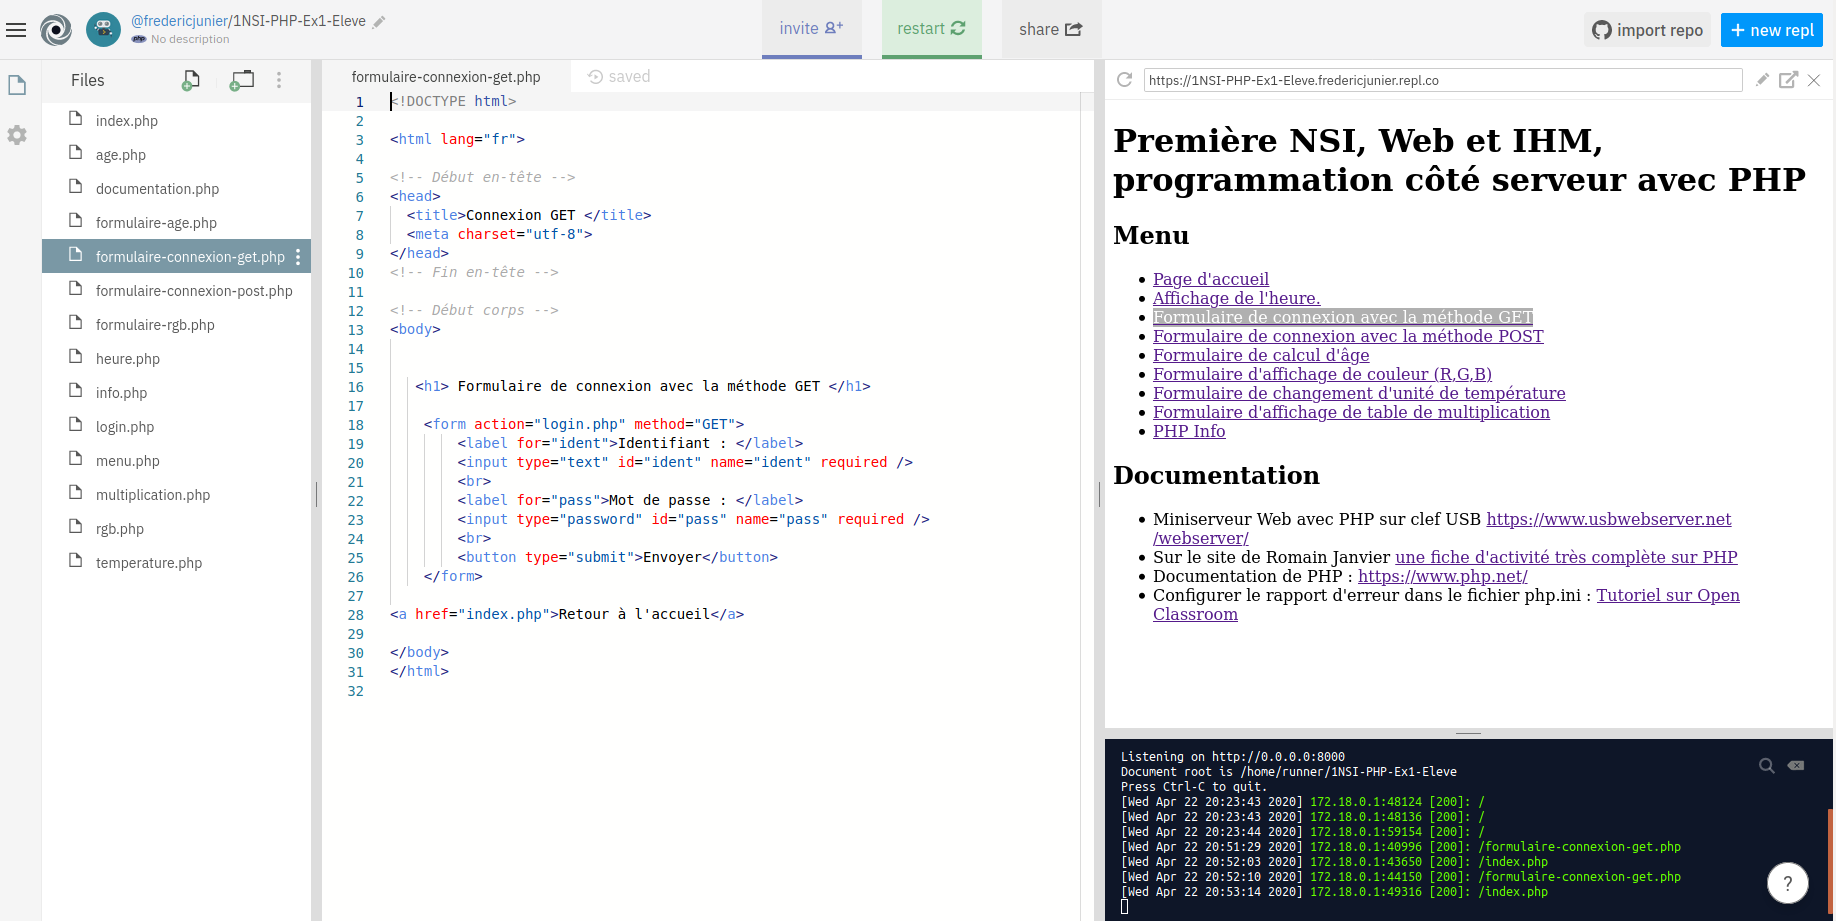
\includegraphics{images/interface-replit.png}~

\begin{enumerate}
\def\labelenumi{\arabic{enumi}.}
\item
  Dans la page d'accueil, cliquer sur le lien \textbf{Formulaire de
  connexion avec la méthode GET}. Remplir le formulaire avec un nom
  quelconque pour l'identifiant et \passthrough{\lstinline!secret!} en
  minuscules pour le mot de passe. Réaliser un autre envoi avec un mot
  de passe incorrect. Le code source du formulaire est affiché dans la
  zone d'édition de l'image précédente. Les dpnnées du formulaire sont
  envoyées par la méthode
  \href{https://developer.mozilla.org/fr/docs/Web/HTTP/M\%C3\%A9thode/GET}{GET}
  au programme \passthrough{\lstinline!login.php!} qui va les traiter.
  Cliquer sur \passthrough{\lstinline!login.php!} dans l'explorateur de
  fichier pour afficher son code source comme ci-dessous :

\begin{lstlisting}[language=PHP]
<!DOCTYPE html>

<html lang="fr">

<head>
<title>Affichage de l'âge avec PHP </title>
<meta charset="utf-8">    
</head>

<body>

<div>
<?php
echo "<p> Il est " . date("H:i:s") . "</p>"; 
/* commentaire
multiligne 
*/
if ( isset($_GET['ident']) && isset($_GET['pass']) 
      && ( $_GET['pass'] ==   'secret' ) )
{
   echo "<p> Bienvenue " . $_GET['ident'] . "</p>";
}
elseif ( !( empty($_POST['ident']) || empty($_POST['pass']) ) 
         && ( $_POST['pass'] == 'secret' ) )
{
   echo "<p>Bienvenue " . $_POST['ident'] . "</p>";
}
else 
{
   echo "<p> Échec de la connexion. </p>"; //commentaire isolé
}
?>
</div>

<a href="index.php">Retour à l'accueil</a>

</body>
</html> 
\end{lstlisting}
\item
  On peut relever dans cet exemple quelques traits du langage
  \href{https://developer.mozilla.org/fr/docs/Glossaire/PHP}{PHP}, que
  nous survolerons :

  \begin{itemize}
  \tightlist
  \item
    On l'a déjà dit le code
    \href{https://developer.mozilla.org/fr/docs/Glossaire/PHP}{PHP} peut
    s'insérer dans du code
    \href{https://developer.mozilla.org/fr/docs/Glossaire/HTML}{HTML},
    entre une des balises \passthrough{\lstinline!<?php!} et
    \passthrough{\lstinline!?>!}
  \item
    Chaque instruction se termine par un symbole
    \passthrough{\lstinline!;!}
  \item
    On peut insérer des commentaires multilignes ou isolés.
  \item
    Les noms de variables doivent être préfixés par le symbole
    \passthrough{\lstinline!$!}.
  \item
    \passthrough{\lstinline!$\_GET!} est une variable spéciale qui va
    recevoir des données de formulaire transmises par la méthode
    \passthrough{\lstinline!$\_GET!}. Il existe aussi une variable
    spéciale \passthrough{\lstinline!$\_POST!}. Il s'agit de tableaux
    associatifs comme les dictionnaires en
    \href{https://docs.python.org/3.7/library/cgi.html}{Python}.
  \item
    L'affichage sur la sortie standard du programme se fait avec
    \passthrough{\lstinline!echo!} comme en
    \href{https://doc.ubuntu-fr.org/bash}{Bash}, et les chaînes de
    caractères sont concaténés avec le symbole
    \passthrough{\lstinline!.!}.
  \item
    Les structures de contrôle (conditions et boucles) ont des
    structures et des mots clefs similaires à tous les autres langages
    procéduraux. Contrairement à
    \href{https://docs.python.org/3.7/library/cgi.html}{Python},
    l'indentation n'a qu'une valeur de présentation, les blocs
    d'instructions doivent donc être délimités par des symboles
    \passthrough{\lstinline!\{!} et \passthrough{\lstinline!\}!}.
  \item
    Pour tester si une variable est définie on peut utiliser la fonction
    \passthrough{\lstinline!isset!} ou son contraire
    \passthrough{\lstinline!empty!}.
  \item
    Les opérateurs logiques sont les mêmes qu'en {[}C{]}{[}C{]},
    \passthrough{\lstinline!\&\&!} pour \passthrough{\lstinline!and!},
    \passthrough{\lstinline!||!} pour \passthrough{\lstinline!or!},
    \passthrough{\lstinline"!"} pour \passthrough{\lstinline!not!} et il
    est conseillé d'utiliser des parenthèses pour clarifier l'ordre
    souhaité.
  \end{itemize}
\item
  Si on édite le code source de la page d'accueil
  \passthrough{\lstinline!index.php!}, on peut remarquer des
  instructions
  \href{https://developer.mozilla.org/fr/docs/Glossaire/PHP}{PHP} comme
  \passthrough{\lstinline!<?php include('menu.php') ?>!} et si on édite
  le fichier \passthrough{\lstinline!menu.php!} on y trouve un menu sous
  forme de liste en
  \href{https://developer.mozilla.org/fr/docs/Glossaire/HTML}{HTML}. On
  peut donc utiliser
  \href{https://developer.mozilla.org/fr/docs/Glossaire/PHP}{PHP} comme
  gestionnaire de templates
  \href{https://developer.mozilla.org/fr/docs/Glossaire/HTML}{HTML} et
  centraliser du code.
\end{enumerate}

\end{exemple}

\hypertarget{une-peu-dexercice}{%
\subsection{Une peu d'exercice}\label{une-peu-dexercice}}

\begin{exercice}{}

Ouvrir dans un navigateur Web la page
\url{https://repl.it/@fredericjunier/1NSI-PHP-Ex1-Eleve} présentée dans
l'exemple 1.

\begin{enumerate}
\def\labelenumi{\arabic{enumi}.}
\item
  Éditer le fichier \passthrough{\lstinline!formulaire-age.php!} et
  compléter le formulaire ci-dessous avec un élément
  \passthrough{\lstinline!<input type="number" name="a">!} de type
  \passthrough{\lstinline!number!} pour que l'utilisateur puisse saisir
  une date de naissance comprise entre 1900 et 2020 et que cette valeur
  soit associée au nom \passthrough{\lstinline!a!} et transmise pour
  traitement au script \passthrough{\lstinline!age.php!} avec la méthode
  \href{https://developer.mozilla.org/fr/docs/Web/HTTP/M\%C3\%A9thode/GET}{GET}.

\begin{lstlisting}[language=HTML]
   <form action="age.php" method="GET">
      <label for="naissance">Saisissez votre date de naissance </label> 
      <br>
      <!-- compléter -->
   </form>
\end{lstlisting}

  Tester l'envoir du formulaire puis retourner à la page d'accueil.
\item
  Dans la page d'accueil, cliquer sur le lien \textbf{Formulaire de
  connexion avec la méthode POST}, saisir dans le champ identifiant
  \passthrough{\lstinline"<script>alert('Hack !')</script>"} et dans le
  champ mot de passe \passthrough{\lstinline!secret!} puis envoyer les
  données. Que se passe-t-il ?

  Faire un nouveau test en saisissant
  \passthrough{\lstinline!<script>window.location.href='index.php'</script>!}.
  Que se passe-t-il ?

  Résumer la définition d'une faille Cross-site scripting (XSS) à partir
  de l'article
  \url{https://developer.mozilla.org/fr/docs/Glossaire/Cross-site_scripting}.

  Modifier le code
  \href{https://developer.mozilla.org/fr/docs/Glossaire/PHP}{PHP} du
  fichier \passthrough{\lstinline!login.php!} pour résoudre en partie
  cette faille à l'aide de la fonction
  \passthrough{\lstinline!htmlspecialchars!} présenté dans cet article
  \url{https://www.w3schools.com/php/php_form_validation.asp}.
\item
  Dans la page d'accueil, cliquer sur le lien \textbf{Formulaire
  d'affichage de couleur (R,G,B)}. On arrive sur un formulaire constitué
  de trois champs \passthrough{\lstinline!<input>!} de type
  \passthrough{\lstinline!number!} où l'utilisateur peut saisir l'une
  des composantes (R,G,B) d'une couleur comprise entre 0 et 255. Les
  données sont envoyées au fichier \passthrough{\lstinline!rgb.php!}.
  Éditer ce fichier depuis l'explorateur et le compléter pour qu'il
  puisse traiter les données du formulaire et modifier la propriété
  \href{https://developer.mozilla.org/fr/docs/Glossaire/CSS}{CSS}
  \passthrough{\lstinline!background!} de l'élément
  \passthrough{\lstinline!<div>!} identifié par
  \passthrough{\lstinline!\#couleur!} afin d'afficher la couleur
  correspondante. Les parties de code à compléter sont marquées par des
  commentaires.

  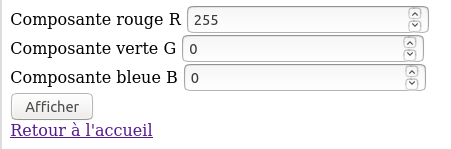
\includegraphics[width=0.5\textwidth,height=\textheight]{images/formulaire_rgb.png}~

  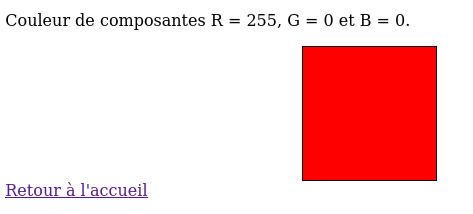
\includegraphics[width=0.5\textwidth,height=\textheight]{images/couleur_rgb.png}~
\item
  Dans la page d'accueil, cliquer sur le lien \textbf{Formulaire de
  changement d'unité de température}. On arrive sur un formulaire
  \passthrough{\lstinline!temperature.php!} constitué d'un champ
  \passthrough{\lstinline!<select>!} permettant de choisir une unité
  source et un champ \passthrough{\lstinline!<input>!} de type
  \passthrough{\lstinline!number!} pour saisir une mesure de
  température. Les données du formulaire sont envoyées à
  \passthrough{\lstinline!temperature.php!} qui supporte donc à la fois
  la saisie et le traitement des données. Éditer ce fichier depuis
  l'explorateur et le compléter pour qu'il puisse traiter les données du
  formulaire en convertissant la mesure de température de Celsius en
  Fahrenheit ou réciproquement.

  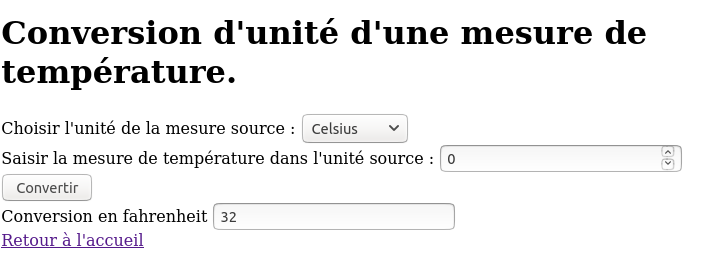
\includegraphics[width=0.5\textwidth,height=\textheight]{images/conversion_unite.png}~
\item
  Dans la page d'accueil, cliquer sur le lien \textbf{Formulaire
  d'affichage de table de multiplication}. On arrive sur un formulaire
  \passthrough{\lstinline!multiplication.php!} constitué d'un champ
  champ \passthrough{\lstinline!<input>!} de type
  \passthrough{\lstinline!number!} pour saisir un facteur. Les données
  du formulaire sont envoyées au même fichier
  \passthrough{\lstinline!multiplication.php!}. Éditer ce fichier depuis
  l'explorateur et le compléter pour qu'il puisse traiter les données du
  formulaire en affichant la table des 11 premiers multiples du nombre
  choisi.

  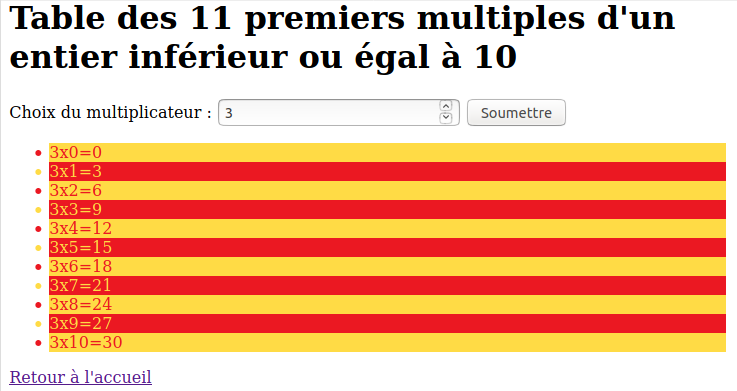
\includegraphics[width=0.5\textwidth,height=\textheight]{images/multiplication.png}~
\end{enumerate}

\end{exercice}

\begin{exercice}{}

\emph{QCM} de type E3C2.

\begin{enumerate}
\def\labelenumi{\arabic{enumi}.}
\item
  Parmi les quatre propositions suivantes, laquelle est la seule à
  correspondre à un entête correct de formulaire d'une page HTML ?

  \begin{itemize}
  \tightlist
  \item
    Réponse A :
    \passthrough{\lstinline!<form method="formulaire.php" action="submit">!}
  \item
    Réponse B :
    \passthrough{\lstinline!<form method="post" action=onclick()>!}
  \item
    Réponse C :
    \passthrough{\lstinline!<form method="get" action="arret.php">!}
  \item
    Réponse D :
    \passthrough{\lstinline!<form method="post" action=arret.php>!}
  \end{itemize}
\item
  Quel langage est interprété ou exécuté côté serveur ?

  \begin{itemize}
  \tightlist
  \item
    Réponse A : JavaScript
  \item
    Réponse B : PHP
  \item
    Réponse C : HTML
  \item
    Réponse D : CSS
  \end{itemize}
\item
  Pour analyser les réponses saisies par l'utilisateur dans un
  formulaire d'une page Web personnelle, hébergée chez unfournisseur
  d'accès à internet, on dispose du code suivant :

\begin{lstlisting}[language=PHP]
<?php if ($_POST['choix']=='choix4'){echo 'Bravo,';}
else {echo "Non, vous vous trompez !";}
?>
\end{lstlisting}

  Où s'exécutera ce code~?

  \begin{itemize}
  \tightlist
  \item
    Réponse A : dans le premier routeur permettant d'accéder au serveur
  \item
    Réponse B : dans le dernier routeur permettant d'accéder au serveur
  \item
    Réponse C : dans le serveur qui héberge la page personnelle
  \item
    Réponse D : dans la machine de l'utilisateur qui consulte la page
    personnelle
  \end{itemize}
\item
  Le site internet d'un quotidien d'information permet aux visiteurs de
  laisser des commentaires textuels. Ces commentaires doivent être
  visibles par les autres visiteurs. Laquelle des affirmations suivantes
  est correcte~?

  \begin{itemize}
  \tightlist
  \item
    Réponse A : Il suffit que la page HTML contienne des champs de la
    forme \passthrough{\lstinline!<textarea>!}
  \item
    Réponse B : Il suffit que la page HTML contienne des champs de la
    forme \passthrough{\lstinline!<textarea>!} et d'utiliser JavaScript
    pour enregistrer les commentaires
  \item
    Réponse C : Il faut un programme en PHP ou un script Python sur le
    serveur pour traiter les données
  \item
    Réponse D : Non, ce n'est pas possible avec la technologie actuelle
  \end{itemize}
\item
  Dans quels langages les balises \passthrough{\lstinline!<img>!} et
  \passthrough{\lstinline!<form>!} sont-elles utilisées~?

  \begin{itemize}
  \tightlist
  \item
    Réponse A : Python
  \item
    Réponse B : HTML
  \item
    Réponse C : Javascript
  \item
    Réponse D : PHP
  \end{itemize}
\end{enumerate}

\end{exercice}

\hypertarget{duxe9veloppement-cuxf4tuxe9-serveur-en-python}{%
\section{Développement côté serveur en
Python}\label{duxe9veloppement-cuxf4tuxe9-serveur-en-python}}

\hypertarget{un-premier-exemple-1}{%
\subsection{Un premier exemple}\label{un-premier-exemple-1}}

\begin{exemple}{}

\href{https://flask.palletsprojects.com/en/1.1.x/}{Flask} est un micro
\href{https://fr.wikipedia.org/wiki/Framework}{Framework} permettant de
développer des applications Web en
\href{https://docs.python.org/3.7/library/cgi.html}{Python}. Il impose
peu de choix prédéfinis au programmeur.

\begin{enumerate}
\def\labelenumi{\arabic{enumi}.}
\item
  Ouvrir dans un navigateur Web la page
  d'\href{https://developer.mozilla.org/fr/docs/Glossaire/URL}{URL}
  \url{https://repl.it/@fredericjunier/1NSI-Flask-Ex1-Eleve-1}.
\item
  On arrive sur un environnement de programmation Web intégrant une mini
  application écrite avec
  \href{https://flask.palletsprojects.com/en/1.1.x/}{Flask}.

  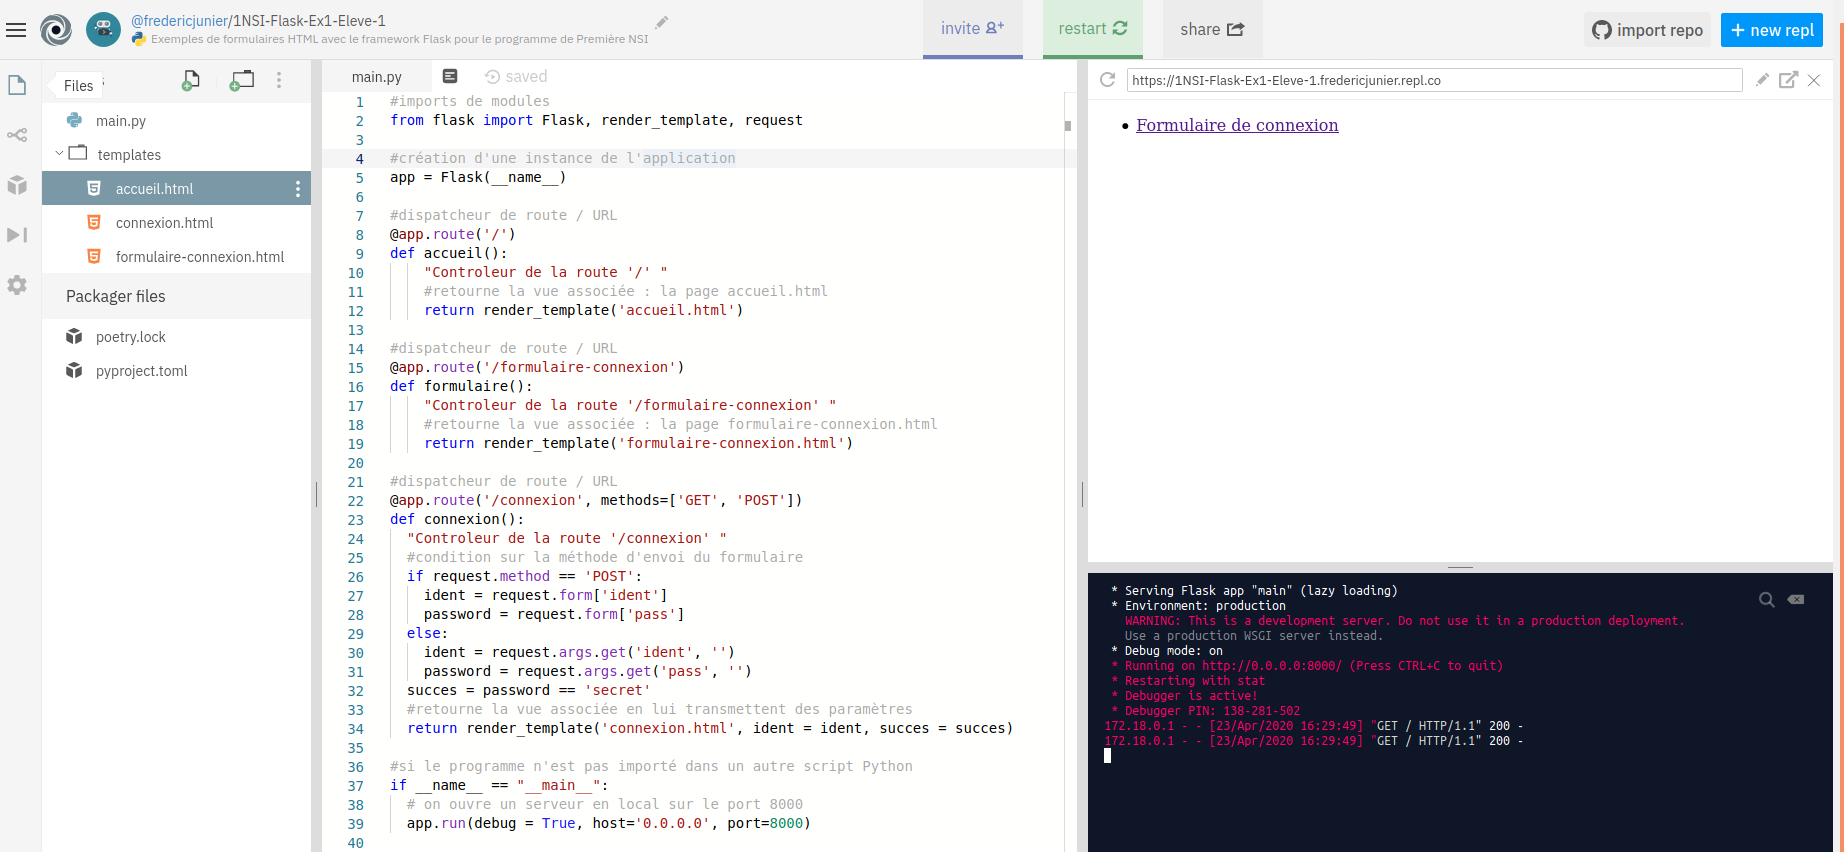
\includegraphics{images/flask-exemple1.png}\\

  \begin{itemize}
  \item
    Tout le code
    \href{https://docs.python.org/3.7/library/cgi.html}{Python} de
    l'application est rassemblé dans le fichier
    \passthrough{\lstinline!main.py!} ouvert dans l'éditeur :
  \item
    On importe d'abord les modules nécessaires avec
    \passthrough{\lstinline!import!}
  \item
    A la fin du programme, un serveur Web de développement est lancé
    avec le débogueur activé.
  \item
    Entre les deux, on trouve une série de déclarations de fonctions
    précédées du décorateur \passthrough{\lstinline!@app.route!}. Le
    décorateur est le \emph{routeur} : si
    l'\href{https://developer.mozilla.org/fr/docs/Glossaire/URL}{URL} se
    termine par \passthrough{\lstinline!/!}, la fonction
    \passthrough{\lstinline!accueil!} est appelée et celle-ci affiche la
    page \passthrough{\lstinline!accueil.html!} par un appel à
    \passthrough{\lstinline!render\_template!}. On parle de \emph{route}
    pour la partie de
    l'\href{https://developer.mozilla.org/fr/docs/Glossaire/URL}{URL}
    correspondant au chemin relatif dans l'application. La fonction
    \passthrough{\lstinline!accueil!} est un \emph{contrôleur} et le
    template
    \href{https://developer.mozilla.org/fr/docs/Glossaire/HTML}{HTML}
    est une \emph{vue} si on refère au modèle d'architecture logicielle
    \href{https://developer.mozilla.org/fr/docs/Glossaire/MVC}{MVC} pour
    \emph{Modèle Vue Contrôleur}.

\begin{lstlisting}[language=Python]
#dispatcheur de route / URL
@app.route('/')
def accueil():
   "Controleur de la route '/' "
   #retourne la vue associée : la page accueil.html
   return render_template('accueil.html')
\end{lstlisting}

    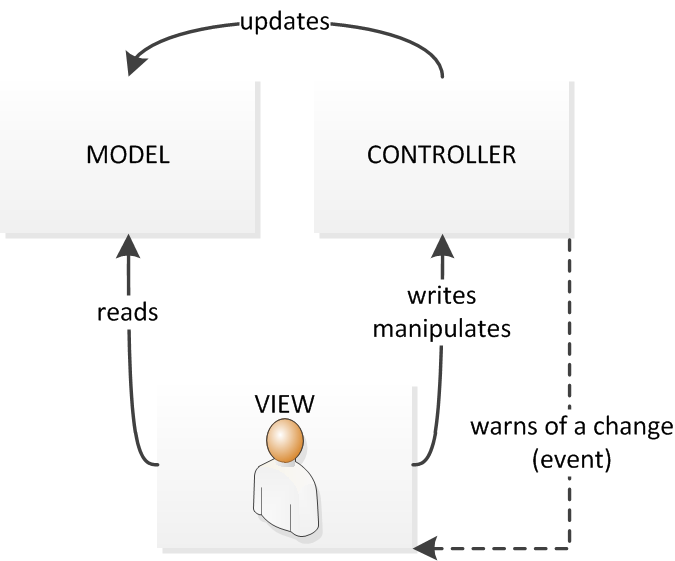
\includegraphics{images/ModeleMVC.png}\\
  \item
    Le code
    \href{https://developer.mozilla.org/fr/docs/Glossaire/HTML}{HTML} de
    la page d'accueil est donné ci-dessous. Si on suit le lien
    hypertexte, d'après la règle de routage définie dans
    \passthrough{\lstinline!main.py!}, le contrôleur
    \passthrough{\lstinline!formulaire!} est appelé et il retourne la
    vue \passthrough{\lstinline!formulaire-connexion.html!} qui est le
    même formulaire de connexion avec deux champs
    \passthrough{\lstinline!ident!} pour l'identifiant et
    \passthrough{\lstinline!pass!} pour le mot de passe que dans
    l'exemple 1 traité avec
    \href{https://developer.mozilla.org/fr/docs/Glossaire/PHP}{PHP}.

\begin{lstlisting}[language=HTML]
<!DOCTYPE html>
<html>
   <head>
      <title> Accueil </title>
      <meta charset="utf-8">
   </head>         
   <body> 
   <a href="/formulaire-connexion"> Formulaire de connexion </a>
   </body>
</html> 
\end{lstlisting}
  \item
    Le formulaire commence par
    \passthrough{\lstinline!<form action="/connexion" method="POST">!},
    il est paramétré pour appeler la route
    \passthrough{\lstinline!/connexion!} qui est associée au contrôleur
    \passthrough{\lstinline!connexion!}. On peut noter que toute la
    logique de contrôle des paramètres est rassemblée ici alors qu'avec
    \href{https://developer.mozilla.org/fr/docs/Glossaire/PHP}{PHP},
    elle était mélangée avec le code de la vue en
    \href{https://developer.mozilla.org/fr/docs/Glossaire/HTML}{HTML}.

\begin{lstlisting}[language=Python]
   @app.route('/connexion', methods=['GET', 'POST'])
   def connexion():
      "Controleur de la route '/connexion' "
      #si la méthode est POST
      if request.method == 'POST':
         #les valeurs des paramètres sont dans le dictionnaire request.form 
         ident = request.form['ident']
         password = request.form['pass']    
      else: #sinon c'est GET
         #la chaine de  paramètres est dans le dictionnaire request.args
         ident = request.args.get('ident', '') 
         password = request.args.get('pass', '')
      succes = password == 'secret'
      #retourne la vue associée en lui transmettant des paramètres
      return render_template('connexion.html', ident = ident, succes = succes)
\end{lstlisting}
  \item
    On peut se demander comment les paramètres sont intégrés au code
    \href{https://developer.mozilla.org/fr/docs/Glossaire/HTML}{HTML} de
    \passthrough{\lstinline!connexion.html!}. Si on édite ce fichier, on
    observe des balises particulières délimitées par des accolades pour
    insérer les paramètres et \passthrough{\lstinline!ident!} et
    \passthrough{\lstinline!succes!} et exécuter uen structure
    conditionnelle.
    \href{https://flask.palletsprojects.com/en/1.1.x/}{Flask} utiliser
    le moteur de template
    \href{https://jinja.palletsprojects.com/en/2.11.x/}{Jinja} pour
    personnaliser des templates
    \href{https://developer.mozilla.org/fr/docs/Glossaire/HTML}{HTML}.

\begin{lstlisting}
~~~html
   <!DOCTYPE html>
      <html>
      <head>
      <title> Page de connexion </title>
      <meta charset="utf-8">   
      </head>  
      <body>   
      
         <h1> Bonjour {{ ident }} </h1>
      
         <h1> Erreur de connexion </h1>
      
      <a href="/">Retour à l'accueil</a>
      </body>
      </html> 
~~~
\end{lstlisting}
  \item
    On peut effectuer quelques tests en changeant la méthode de passage
    des paramètres dans le formulaire de connexion pour s'assurer que le
    contrôleur fonctionne bien.
  \item
    Si on simule une attaque XSS en saisissant du code
    \href{https://developer.mozilla.org/fr/docs/Glossaire/JavaScript}{Javascript}
    dans le champ d'identifiant :
    \passthrough{\lstinline!<script>alert("Hack")</script>!}, on peut
    observer que le moteur de template échappe par défaut les caractères
    spéciaux
    \href{https://developer.mozilla.org/fr/docs/Glossaire/HTML}{HTML}
  \end{itemize}
\item
  Pour résumer,
  \href{https://flask.palletsprojects.com/en/1.1.x/}{Flask} permet de
  développer une application côté serveur comme
  \href{https://developer.mozilla.org/fr/docs/Glossaire/PHP}{PHP} mais,
  en première approche, il offre une séparation plus lisible entre la
  logique de l'application dans un fichier
  \href{https://docs.python.org/3.7/library/cgi.html}{Python} et
  l'affichage dans des fichiers
  \href{https://developer.mozilla.org/fr/docs/Glossaire/HTML}{HTML}.
\end{enumerate}

\end{exemple}

\hypertarget{un-peu-dexercice}{%
\subsection{Un peu d'exercice}\label{un-peu-dexercice}}

\begin{exercice}{}

\begin{enumerate}
\def\labelenumi{\arabic{enumi}.}
\item
  Ouvrir dans un navigateur Web la page
  d'\href{https://developer.mozilla.org/fr/docs/Glossaire/URL}{URL}
  \url{https://repl.it/@fredericjunier/1NSI-Flask-Ex2-Eleve}.
\item
  On arrive sur un environnement de programmation Web intégrant une mini
  application écrite avec
  \href{https://flask.palletsprojects.com/en/1.1.x/}{Flask}. Le fichier
  \passthrough{\lstinline!main.py!} contient le moteur de l'application.

  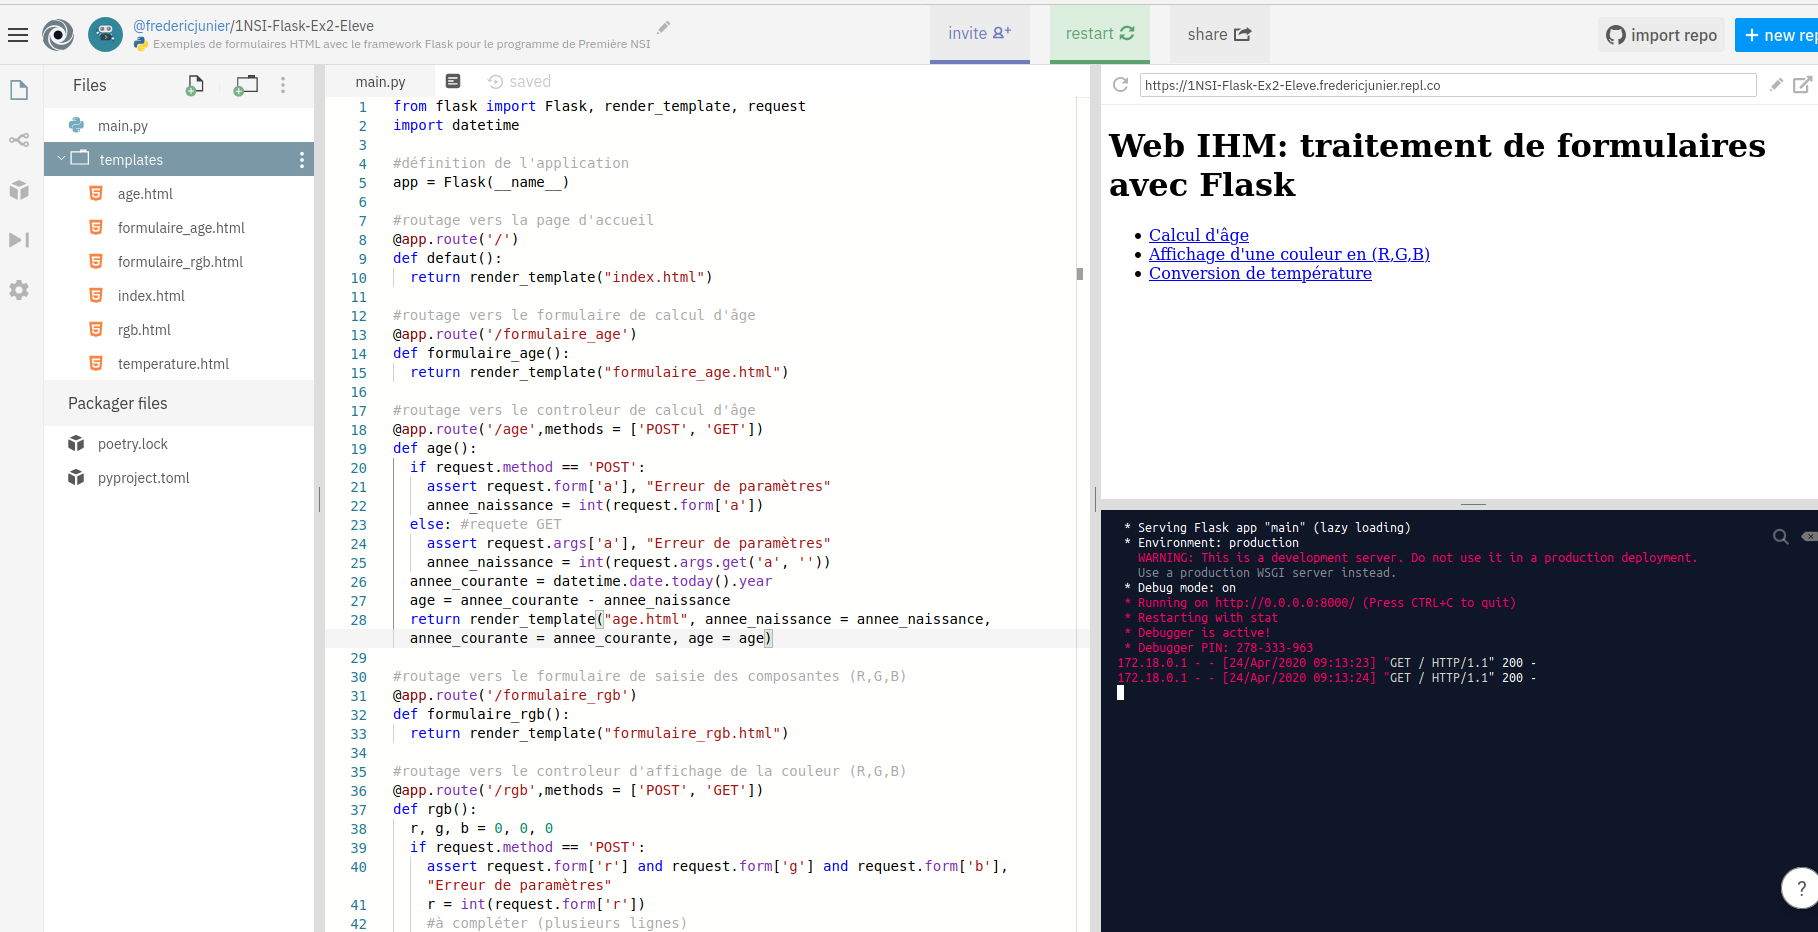
\includegraphics{images/flask-exemple2.png}\\
\item
  Éditer le code source de la page d'accueil
  \passthrough{\lstinline!accueil.html!} de l'application. Elle contient
  trois liens vers des formulaires :

  \begin{itemize}
  \tightlist
  \item
    Calcul d'âge\\
  \item
    Affichage d'une couleur en (R,G,B)
  \item
    Conversion de température \footnote{Note : ce formulaire renvoie
      vers lui-même}
  \end{itemize}
\item
  Compléter le code de \passthrough{\lstinline!main.py!} aux
  emplacements marqués par un commentaire
  \passthrough{\lstinline!\# à compléter!} pour obtenir le même
  comportement que les formulaires éponymes contenus dans l'exercice 1
  réalisé avec
  \href{https://developer.mozilla.org/fr/docs/Glossaire/PHP}{PHP} :
  \url{https://repl.it/@fredericjunier/1NSI-PHP-Ex1-Correction}. Tester
  les formulaires en modifiant les méthodes de passage des paramètres
  pour que les trois formulaires fonctionnent avec
  \href{https://developer.mozilla.org/fr/docs/Web/HTTP/M\%C3\%A9thode/POST}{POST}
  ou
  \href{https://developer.mozilla.org/fr/docs/Web/HTTP/M\%C3\%A9thode/GET}{GET}.
\end{enumerate}

\end{exercice}

\end{document}
